\documentclass[a4paper]{article}

\usepackage{graphicx}
\usepackage{xcolor}
\usepackage{hyperref}
\usepackage{amsfonts}
\usepackage{mathtools}
\usepackage{subcaption}
\usepackage{float}

\graphicspath{{../images/}}


\title{Course Project}
\author{aiman-haq \and muhammadhamza23 \and shaikh-fahad}
\date{CS 412 Algorithms: Design and Analysis\\Spring 2022}

\begin{document}
\maketitle

\section{Introduction}
This proposal serves the purpose of indicating a computational problem for which algorithmic solutions are found and, or devised, each of which corresponds to a distinct algorithmic paradigm/design technique.

\noindent
Before moving onto the chosen problem and its range of solutions, let us first look at some other salient information with respect to the project.

\subsection{Working Title}
The project shall proceed under the following working title, \emph{\textbf{Nodi Connectome}}.

\subsection{Group Composition}
The team undertaking this course project is known as \emph{\textbf{planar-analysis}} and its members (\textit{find} \texttt{GitHub} \textit{IDs listed above}) are as follows:
\begin{itemize}
    \item Aiman Haq, \href{mailto:ah04318@st.habib.edu.pk}{ah04318@st.habib.edu.pk}
    \item Syed Muhammad Hamza, \href{mailto:sh05192@st.habib.edu.pk}{sh05192@st.habib.edu.pk}
    \item Fahad Shaikh, \href{mailto:fs05452@st.habib.edu.pk}{fs05452@st.habib.edu.pk}
\end{itemize}

\section{The Problem}
This particular project shall concern itself with the \textbf{Shortest Path Problem}. Intuitively speaking, the problem in question asceratins that given a \emph{source} and a \emph{destination}, what is the Shortest path between them. More formally, such a problem deals with a directed graph,
$G = (V, E)$, with weighted edges that is, it houses a weigh function $w: E \rightarrow \mathbb{R}$ mapping edges to real-valued weights (i.e., costs/distances - these weights represent any metric that accumulates linearly along a path and that we would want to minimize). Now given, such a graph,
the typical objective for finding the shortest path between any two vertices, say $u$ and $v$, is to identiffy a path, $u \xrightarrow{p} v$, in the graph such that the sum of the weights of its consituent edges is minimized \cite{cormenBk,open-dsa,chumbley}- \textbf{Figure} \ref{fig:short-path} illustrates this concept.

\begin{figure}[H]
    \begin{center}
      \begin{subfigure}{.5\textwidth}
        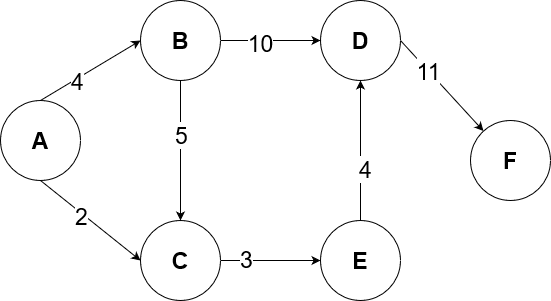
\includegraphics[width=1.75in]{shortest_path_original.png}
        \caption{}
      \end{subfigure}%
      \begin{subfigure}{.4\textwidth}
        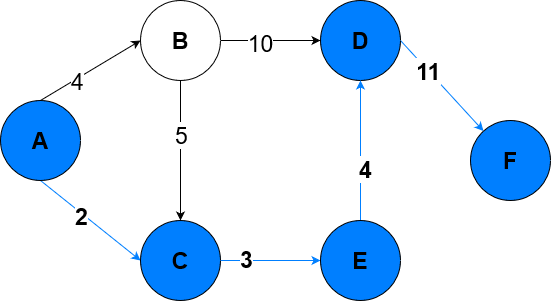
\includegraphics[width=1.75in]{shortest_path_solved.png}
        \caption{}
      \end{subfigure}
    \end{center}
    \caption{Illustrates the concept of a shortest path given a source and a destination. \textbf{(a)} shows the original directed graph. \textbf{(b)} identifies the shortest-path (\emph{edges and nodes marked in \textcolor{blue}{blue}}) for $A \xrightarrow{p} F$.\cite{wikipediaImg}}
    \label{fig:short-path}
\end{figure}


\noindent
Having established the shortest path problem as a whole, let us now reveal a slight obfuscation with respect to the scope of the project. Indeed, the project focuses upon the Shortest Path Problem but what was omitted earlier was the intent to focus solely upon the \textbf{Single-Source Shortest Path}
variant. The decision of dealing prime focus to this particular variant originates from the fact the solution to this specific problem in itself solves many other problems in addition to solving the other variants of the Shortest Path problem \cite{cormenBk,sedgewickBk}:

\begin{enumerate}
    \item Single-destination
    \item Single-pair
    \item All-pairs
\end{enumerate}

\noindent
For a graph, $G = (V, E)$, the \textbf{Single-Source Shortest Path} (SSSP) problem consists of finding the shortest paths between a given \textbf{\emph{source}} vertex $s \in V$ to each vertex $v \in V$ \cite{cormenBk,chaupis-et.al:2017}. \textbf{Figure} \ref{fig:single-soruce} illustrates this concept.

\begin{figure}[H]
    \begin{center}
      \begin{subfigure}{.5\textwidth}
        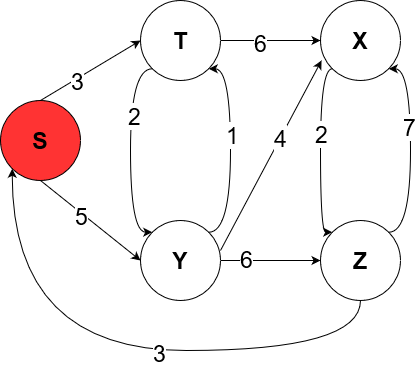
\includegraphics[width=1.75in]{single_source_original.png}
        \caption{}
      \end{subfigure}%
      \begin{subfigure}{.4\textwidth}
        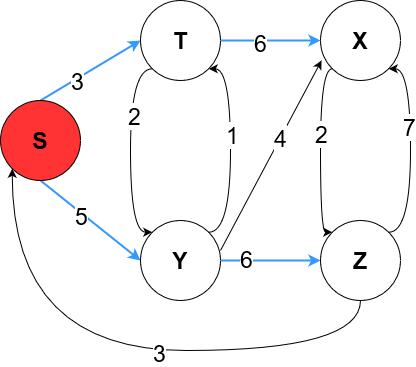
\includegraphics[width=1.75in]{single_source_solved.png}
        \caption{}
      \end{subfigure}
    \end{center}
    \caption{Given a \textbf{source} vertex \(S\), \textbf{(a)} shows the original weighted directed graph with the source vertex marked in \textcolor{red}{red}. \textbf{(b)} shows the same graph from (a) but with the shortest path from the source to every other vertex marked in \textcolor{blue}{blue} - \textbf{Note}: these marked shortest paths are \emph{not unique} (for $S \xrightarrow{p} X$, we have the same minimally costing path if we took the edges \((S, Y), (Y, X)\) as well).\cite{cormenBk}}
    \label{fig:single-soruce}
\end{figure}

\section{Algorithms/Design Techniques}
The project will be focusing on two algorithmic paradigms/design techniques to solve the problem in question. We will considering a \textbf{greedy approach} (i.e., \textit{Dijkstra's algorithm}) and a \textbf{dynamic-programming approach} (i.e., \textit{Bellman-Ford algorithm}).
In later phases of the project, we shall compare both these approaches for the given problem both, theoretically (i.e., \emph{asymptotically}) and empirically.

\subsection{Dijkstra's algorithm}
With Dijkstra's algorithm we generate a shortest path tree with a given source as a root. We maintain two sets, one set contains vertices included in the shortest-path tree, other set includes vertices not yet included in the shortest-path tree. At every step of the algorithm, we find a vertex that is in the other set (set of not yet included) and has a minimum distance from the source.
At the end, we end up with the shortest paths from the source vertex to all other vertices in the graph \cite{dijkstraG4G,dijkstraProgrammiz,huang-et.al:2009}.

\subsection{Bellman-Ford algorithm}
The Bellman-Ford algorithm solves the single-source shortest-paths problem in the general case in which \emph{edge weights may be negative}. The algorithm works by overestimating the length of the path from the starting vertex to all other vertices. Then it iteratively relaxes those estimates by finding new paths that are shorter than the previously overestimated paths.
Like other \textbf{dynamic programming} problems, the algorithm calculates shortest paths in a \emph{bottom-up} manner. It first calculates the shortest distances which have at most one edge in the path. Then, it calculates the shortest paths with at most $2$ edges, and so on. The idea is, assuming that there is no negative weight cycle, if we have calculated shortest paths with at most \(i\) edges, then an iteration over all edges guarantees to give shortest path with at most $(i+1)$ edges \cite{bFordG4G,bFordProgrammiz}.

\newpage
\bibliographystyle{plain} % We choose the "plain" reference style
\bibliography{../refs}

\end{document}
